\documentclass{article}
\usepackage{graphicx}

\title{Homework 2}
\author{Igor Alentev}
\date{\date{\today}}

\begin{document}

\maketitle
\newpage

\section*{Task1}
\subsection*{Simulation Process}

The process was quite the same as the previous time.
I had to implement one-step callback for the path following controller,
as well as initializer. I have entered the required path and parameters.

There are only two differences:

\begin{itemize}
    \item First of all to simplify the cpu load I 
have decided to check trajectories via rviz and not via gazebo.
    \item Secondly, I have decided to publish the required trajectory
    to simplify analysis and debugging of results.
\end{itemize}
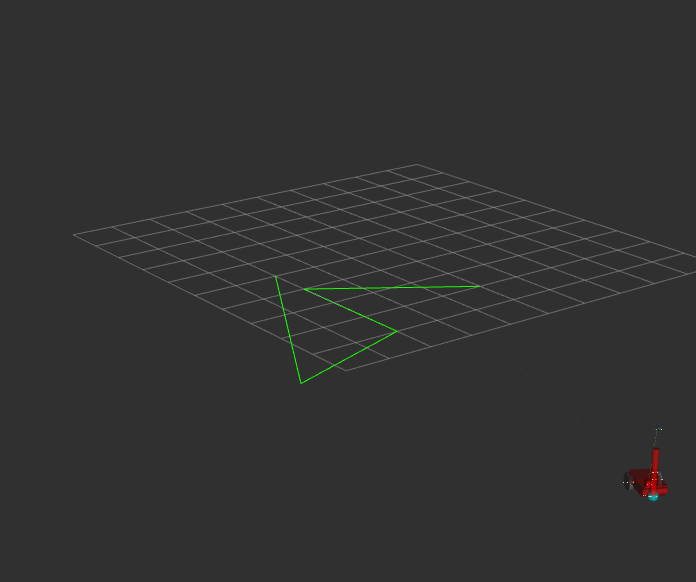
\includegraphics[scale=0.67]{assets/rviz.png}

All what is left is only to implement the simple controller, which we 
have discussed in the class. The only issue I had to debug was that
I have forgotten to wrap to $\pi$ the $\Phi_{err}$.

\subsection*{Results \& Analysis}
Simualation result can be seen on the following figure:

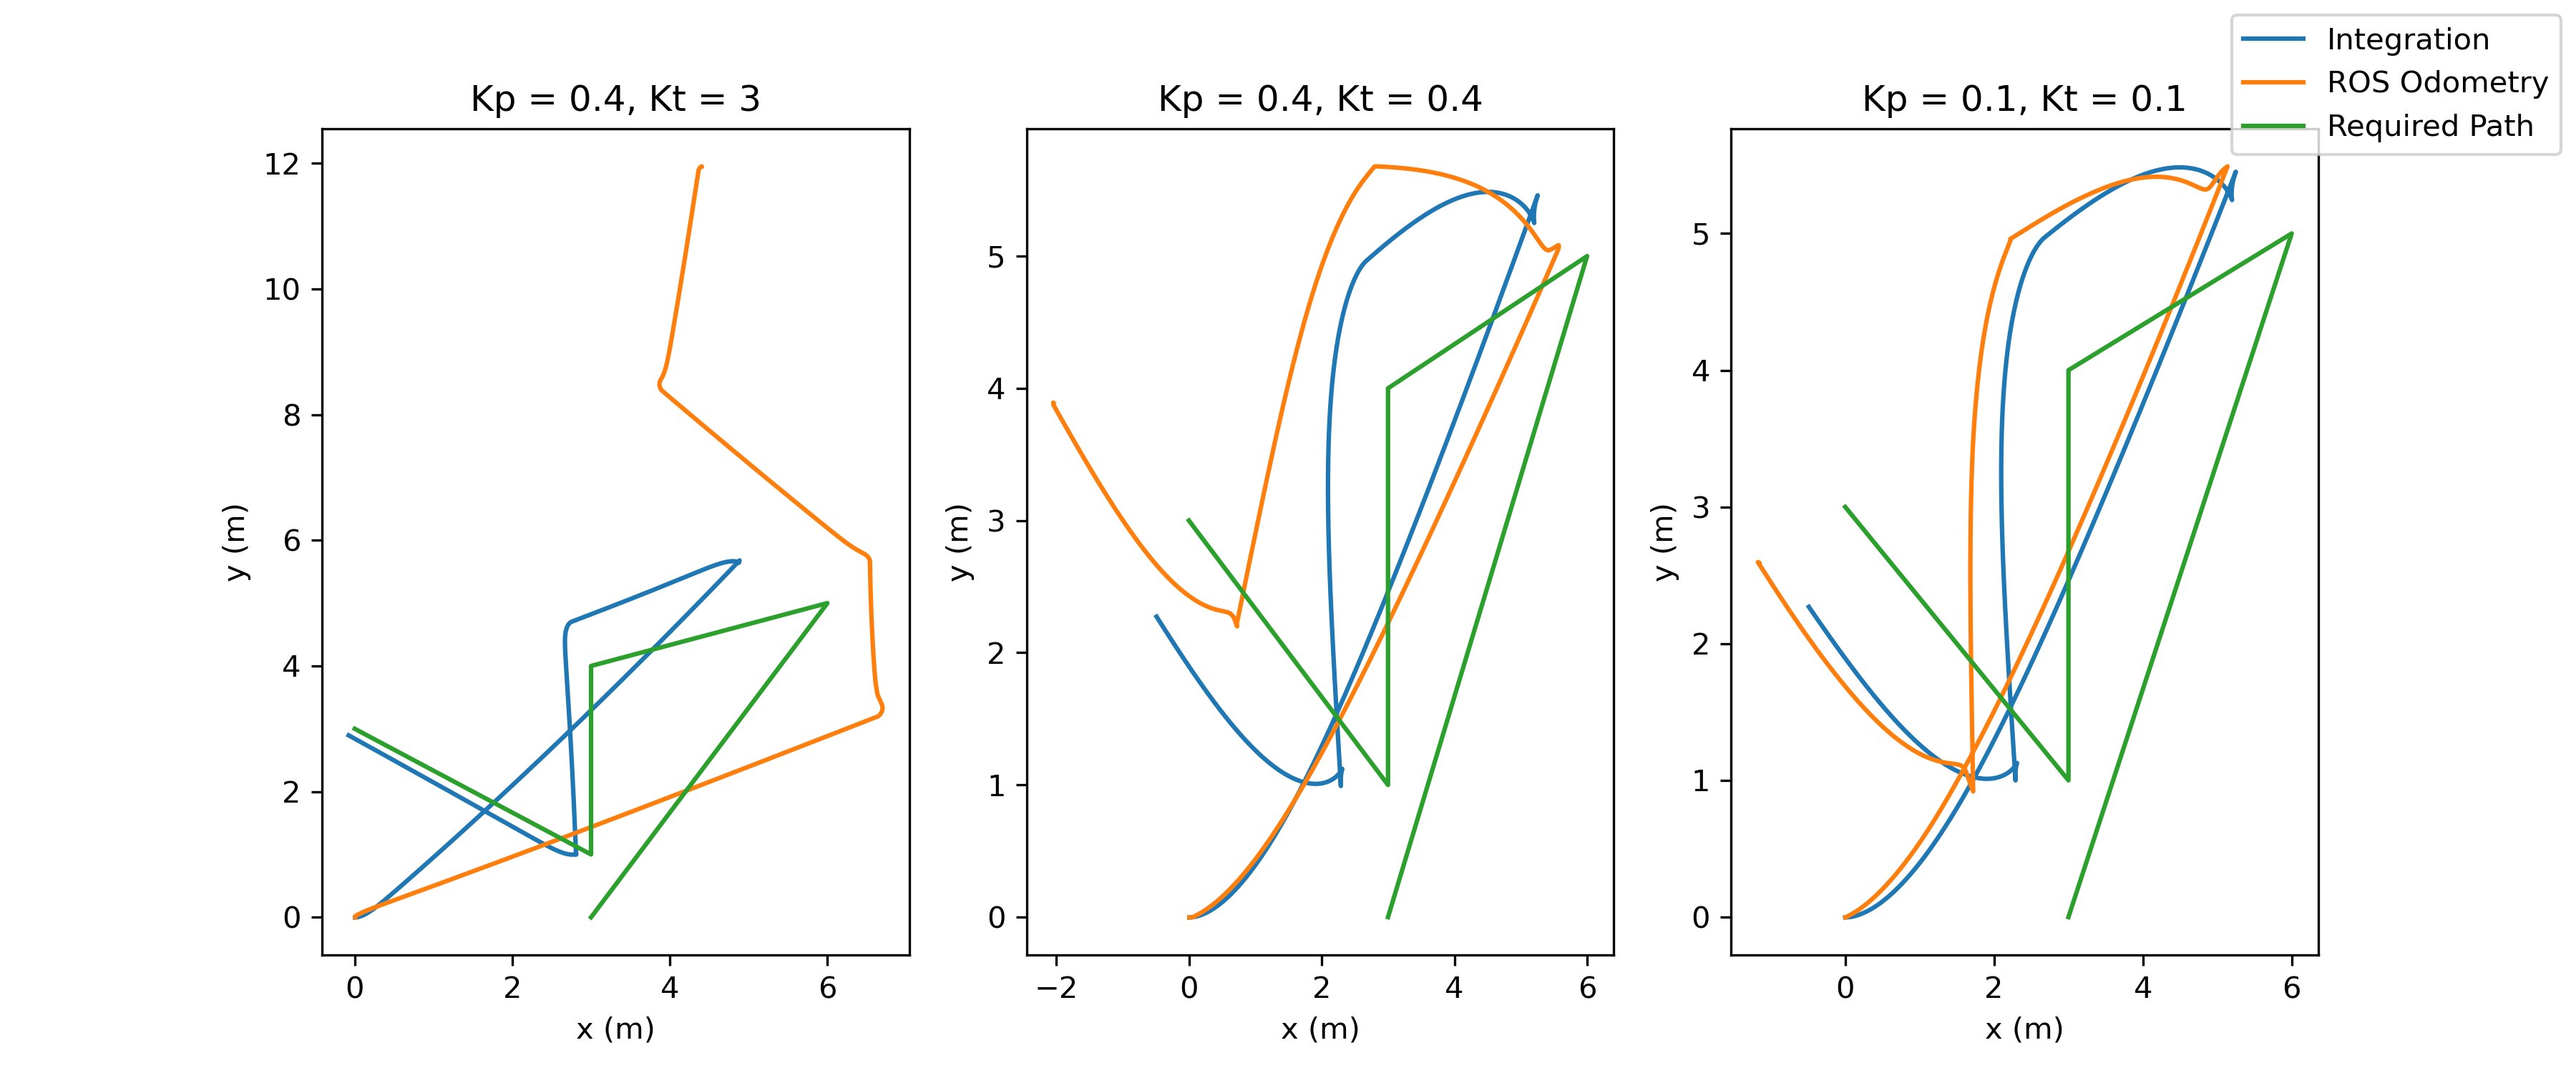
\includegraphics[scale=0.4]{assets/trajectory.png}

\begin{enumerate}
    \item The robot was simulated with the values of $K_p=0.4, K_{\theta}=3$ and was not able to converge to the needed path.
    \item The robot was simulated with the values of $K_p=0.4, K_{\theta}=0.4$ and has a slight error.
    \item The robot was simulated with the values of $K_p=0.1, K_{\theta}=0.1$ and almost completely converges to simualtion path. 
    Even though it has some error if we compare it to the required path.
\end{enumerate}

There might be several reasons for the error and I believe that they are
practically identical to those from previous homework.

However, the issue that numerical integration does not converge to the real 
result is quite interesting. From the graphs we can see, that it happens
if we change the value of angle too quickly. From the logs it could be seen
that numerical integration believes that we have already reached the goal
orientation, even though it did not happen. 

I tend to think that the issue is that we again do not consider the physical 
properties of our robot. Having too high value of $K_{\theta}$ we are rotating
the robot too fast and it is not able to follow the rotation when we simulate
with physics, rather than assuming that the robot is a point.

Lowering the speed of rotation, we are able to follow the path more accurately, basically
the numerical integration is able to follow the real robot as can be seen on the third figure. ($K_p=0.1, K_{\theta}=0.1$)

However, the real robot is unable now to follow the reference trajectory precisely.
I think that it is due to physical properties of the robot. It simply can not
follow the path more precisely without more advanced control.

\end{document}